\chapter{Proposed system}
\label{sec:proposed system}

\section{Overview}
A distributed system where a user is able to search and find movies. Information for the selected movie is displayed. He is able to add the found movie to his favourites list.

\section{Functional requirements}
\begin{itemize}
	\setlength{\itemsep}{-5pt}
	\item The following components shall be implemented
	\begin{itemize}
		\setlength{\itemsep}{-5pt}
		\item A database
		\item A server exposing functions for retrieving data from the database
		\item A Windows Application
		\item A Web Client
	\end{itemize}
	\item All above parts shall be implemented in C\#. The Windows client in WPF and the web client in ASP.NET
	\item Communication between clients and server shall happen in a RESTful manner sending JSON over HTTP
	\item The server must build on the HttpListener for HTTP communication
	\item The server should support two ways of retrieving data. One being from its memory cache and the other being from the Database. If the requested data is in memory it will be retrieved from there instead of from the Database
	\item The desktop client shall support two ways of storing data. One being XML on the disk, and another being in memory cache.
	\begin{itemize}
			\setlength{\itemsep}{-5pt}
			\item If the client is offline: If the requested data is in memory cache it will be retrieved from there instead of from the disk
			\item If the client is online: If the requested data is in memory cache it will be retrieved from there instead of from the disk. In both cases the client will check-up with the Server to see if it has the most recent version
	\end{itemize}
	\item The server shall be able to merge information from My Movie API. If some data is not stored locally, but is in the My Movie API, it will get the data from there and store it locally.
	\item The system shall allow for user registration and login
\end{itemize}

\section{Nonfunctional requirements}

\begin{itemize}

\item[\textbf{Usability}]
\begin{itemize}
\item A user able to use an internet browser must be able to use the System
\end{itemize}

\vspace{0.2cm}
\item[\textbf{Reliability}]
\begin{itemize}
\item Reliability is a \textit{must} for the system. The user should experience as few software crashes as possible, with a maximum of 2 per day.
\item Restarting the system is acceptable if a software crash does happen
\item The system must not lose data as result of a software crash
\end{itemize}


\vspace{0.2cm}
\item[\textbf{Performance}] 

\hspace{50cm}

\begin{itemize}
\item Minimum requirements
\end{itemize}


\begin{tabular}{|p{2cm}|p{5cm}|p{5cm}|}
\hline  & Desktop Client & Web Client \\ 
\hline Operation System & Windows 7/8 & Webkit2 browser \\
\hline Processor & Intel Core2 Duo T7500 or equivalent & 1.4 GHz Scorpion or equivalent \\ 
\hline Memory & 2gb RAM & 512mb RAM \\ 
\hline Storage & 200mb available & non-applicable \\ 
\hline 
\end{tabular} 

\vspace{0.2cm}

\begin{itemize}
\item The system should support at least 7 concurrent users
\item The server must support storing at least 10 gigabytes of data
\item The maximum latency the user can experience, when his internet is not a bottlenect, must not surpass 5 seconds
\end{itemize}

\vspace{0.2cm}
\item[\textbf{Supportability}]
\begin{itemize}
\item Extensibility
\begin{enumerate}
\item The system should be prepared for implementing more functionality which the logged in user can utilize
\item The system should be prepared for changing storage architecture
\end{enumerate}
\end{itemize}

\vspace{0.2cm}
\item[\textbf{Implementation}]
\begin{itemize}
\item The desktop client will be implemented for the Windows 7/8 operation system
\item The web client will be implemented by ASP.NET MVC
\end{itemize}

\vspace{0.2cm}
\item[\textbf{Interface}]
\begin{itemize}
\item The system shall interact with the My Movie API
\item Initial data for the movie database is made available as a .mdf file
\end{itemize}

\vspace{0.2cm}
\item[\textbf{Packaging}]
\begin{itemize}
\item The back-end server software and database is installed by us
\item The Clients are installed by the end-user
\item The desktop client should be portable and not require any installation
\end{itemize}

\end{itemize}


\section{System models}

\subsection{Scenarios}
In order to specify the use cases in which the user can interact with the program, it is required to initially specify a couple of different scenarios the user can have while utilizing the application.

The following scenarios were set up in order to analyze them:

\begin{center}
	\begin{tabular}{ | l | p{10cm} |  }
		 \hline
		Scenario name & \underline{find movie}  \\ \hline
		Participating Actors & \underline{John} \\ \hline
		Flow of Events & \begin{enumerate}
						\item John wants to find out the name of the actor playing the protagonist in Pulp Fiction. He enter the title in the search field.
						\item John receive information for the movie, such as a list of actors, roles, a description for the movie, rating ect.
						\end{enumerate}
						\\ \hline
						
	\end{tabular}
\end{center}


\begin{center}
	\begin{tabular}{ | l | p{10cm} |  }
		 \hline
		Scenario name & \underline{find actor}  \\ \hline
		Participating Actors & \underline{John} \\ \hline
		Flow of Events & \begin{enumerate}
						\item John liked the performance of Samuel L. Jackson in Pulp Fiction, and wants to find other movies where he stars in. He searches for Samuel L. Jackson and recieves his personal information. Ex. Gender and a list of movis he stairs in.
						\end{enumerate}
						\\ \hline
						
	\end{tabular}
\end{center}}


\begin{center}
	\begin{tabular}{ | l | p{10cm} |  }
		 \hline
		Scenario name & \underline{create account}  \\ \hline
		Participating Actors & \underline{John} \\ \hline
		Flow of Events & \begin{enumerate}
						\item John wants to make a user account so he have the opportunity to make a personal favorite list. He presses Register and is prompted for a the user name and a password for his account and press the OK button. His user is now active.
						\end{enumerate}
						\\ \hline
						
	\end{tabular}
\end{center}}


\begin{center}
	\begin{tabular}{ | l | p{10cm} |  }
		 \hline
		Scenario name & \underline{log in}  \\ \hline
		Participating Actors & \underline{John} \\ \hline
		Flow of Events & \begin{enumerate}
						\item John has now made a user, and he wants to log in. He presses login and enters his login information.
						\end{enumerate}
						\\ \hline
						
	\end{tabular}
\end{center}}


\begin{center}
	\begin{tabular}{ | l | p{10cm} |  }
		 \hline
		Scenario name & \underline{add movie to favourite list}  \\ \hline
		Participating Actors & \underline{John} \\ \hline
		Flow of Events & \begin{enumerate}
						\item John loved Pulp Fiction, so he wants to add it to his favourites list.
						\item He searches and finds the movie, and presses the favourites icon in order to add it. John has added Pulp Fiction to his favourite list.
						\end{enumerate}
						\\ \hline
						
	\end{tabular}
\end{center}}


\begin{center}
	\begin{tabular}{ | l | p{10cm} |  }
		 \hline
		Scenario name & \underline{Edit name of actor}  \\ \hline
		Participating Actors & \underline{George} \\ \hline
		Flow of Events & \begin{enumerate}
						\item The admin, George, has discovered that Will Smith is incorrectly called Woll Smoth, and needs to change the name so it is spelled correctly. He logs into his administrator account, searches for and find woll smoth.
						\item John change the name to Will Smith and enter the save button.
						\end{enumerate}
						\\ \hline
						
	\end{tabular}
\end{center}}


\begin{center}
	\begin{tabular}{ | l | p{10cm} |  }
		 \hline
		Scenario name & \underline{add movie and actor to Data Base}  \\ \hline
		Participating Actors & \underline{George} \\ \hline
		Flow of Events & \begin{enumerate}
						\item The new movie, The Hobbit 3, needs to be added to the database. The admin, George, logs into his administrator account and enter The Hobbit 3 with a description, actors and all other information that fits the movie. He notices that an actor which stair in The Hobbit 3, Hans Lars Christiansen, does not exist in the database. George adds the actor to the database, and makes sure that the new actor is linked to the corresponding movie.
						\end{enumerate}
						\\ \hline
						
	\end{tabular}
\end{center}}


\begin{center}
	\begin{tabular}{ | l | p{10cm} |  }
		 \hline
		Scenario name & \underline{edit movie}  \\ \hline
		Participating Actors & \underline{George} \\ \hline
		Flow of Events & \begin{enumerate}
						\item George notices that he made a mistake when adding 'The Hobbit 3' to the database. He had set the genre to a horror movie.
						\item George logs in to his administrator account and edits the movie genre to fantasy.
						\end{enumerate}
						\\ \hline
						
	\end{tabular}
\end{center}}


\begin{center}
	\begin{tabular}{ | l | p{10cm} |  }
		 \hline
		Scenario name & \underline{delete movie}  \\ \hline
		Participating Actors & \underline{George} \\ \hline
		Flow of Events & \begin{enumerate}
						\item George realises that an incompetent intern has added a fake movie to the database. He promptly deletes it and get a notification that the movie is deleted.
						\end{enumerate}
						\\ \hline
						
	\end{tabular}
\end{center}}


\subsection{Use case model}



\begin{itemize}
	\setlength{\itemsep}{-5pt}
	\item User
	\item Administrator
	\item Server
\end{itemize}

Through the inspection of the scenarios depicted in the Scenario’s section, we have deduced the use cases that the program should be able to support.

The use cases are as follows:

User use cases:
\begin{itemize}
	\setlength{\itemsep}{-5pt}
	\item Find movie
	\item Find actor
	\item Make account
	\item Add to favourites list
	\item Remove from favourites list
	\item View favourites list
	\item Log in to account
	\item Log out from account
\end{itemize}

Administrator use cases:
\begin{itemize}
	\item Add movie
	\item Edit movie information
	\item Delete movie
	\item Add actor
	\item Edit actor information
	\item Delete actor
\end{itemize}

After refining the system design, we have added the following boundary scenarios:
\begin{itemize}
	\setlength{\itemsep}{-5pt}
	
	\item StartWebServer
	\item ShutdownWebServer
	\item ConfigureWebServer
	\item ConnectionLostException
\end{itemize}

\begin{figure}[H]
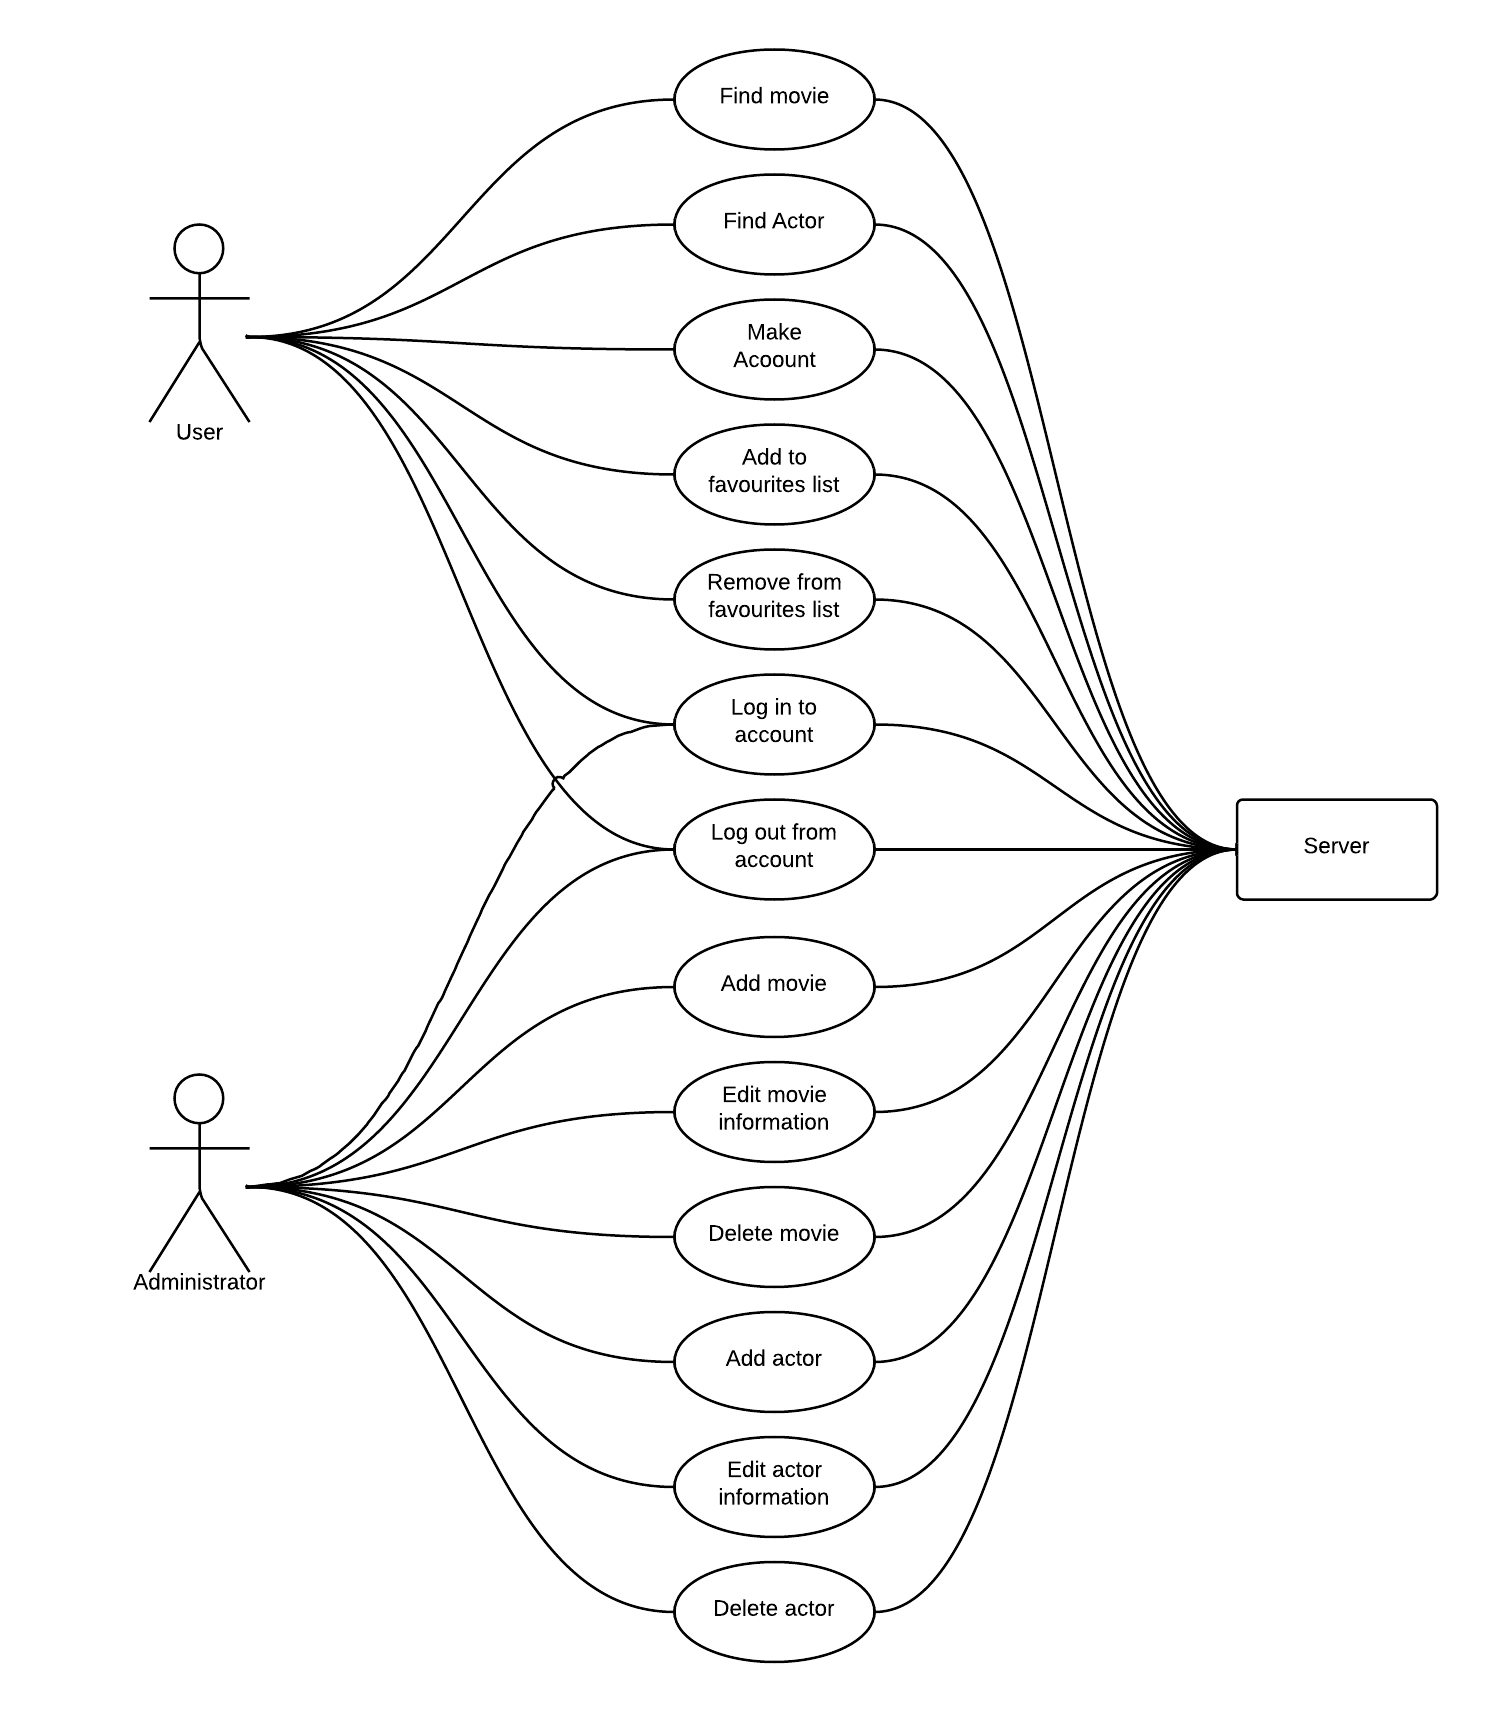
\includegraphics[width=\linewidth]{img/usecasediagram.png}
\caption{Use case diagram}
\label{fig:use case diagram}
\end{figure}

To have a more thorough understanding of each individual use cases, the following explanations was produced, describing each and every step of each use case.
The explanations furthermore include the relation between the actors and the use cases


\begin{center}
	\begin{tabular}{ | l | p{10cm} |  }
		 \hline
		Use Case Name & Find movie \\ \hline
		Participating Actors & Initiated by \emph{User} \\ \hline
		Flow of Events & \begin{enumerate}
						\item[1.] The \emph{user} searches for a movie
						\begin{enumerate}
							\item[2.] The client presents the user with a list of movies with names containing the input
						\end{enumerate}
						\item[3.] The \emph{user} selects one of the search results
						\begin{enumerate}
							\item[4.] The client displays a page containing information on the movie
						\end{enumerate}
					\end{enumerate} \\ \hline
		Entry Condition & \begin{itemize}
						\item The \emph{user} has a client open
					\end{itemize} \\ \hline
		Exit Condition & \begin{itemize}
						\item The \emph{user} successfully found a movie
					\end{itemize} \\
		\hline
	\end{tabular}
\end{center}

\begin{center}
	\begin{tabular}{ | l | p{10cm} |  }
		 \hline
		Use Case Name & Find actor \\ \hline
		Participating Actors & Initiated by \emph{User} \\ \hline
		Flow of Events & \begin{enumerate}
						\item[1.] The \emph{user} searches for an actor
						\begin{enumerate}
							\item[2.] The client presents the user with a list of actors with names containing the input
						\end{enumerate}
						\item[3.] The \emph{user} selects one of the search results
						\begin{enumerate}
							\item[4.] The client displays a page containing information on the actor
						\end{enumerate}
					\end{enumerate} \\ \hline
		Entry Condition & \begin{itemize}
						\item The \emph{user} has a client open
					\end{itemize} \\ \hline
		Exit Condition & \begin{itemize}
						\item The \emph{user} successfully found an actor
					\end{itemize} \\
		\hline
	\end{tabular}
\end{center}

\begin{center}
	\begin{tabular}{ | l | p{10cm} |  }
		 \hline
		Use Case Name & Make account \\ \hline
		Participating Actors & Initiated by \emph{User} \\ \hline
		Flow of Events & \begin{enumerate}
						\item[1.] The \emph{user}, via the client, wishes to create an account
						\begin{enumerate}
							\item[2.] The client presents the user with an account creation page
						\end{enumerate}
						\item[3.] The \emph{user} fills in the required information (username, password)
						\begin{enumerate}
							\item[4.] The client makes the account, and the user is logged in.
						\end{enumerate}
					\end{enumerate} \\ \hline
		Entry Condition & \begin{itemize}
						\item The \emph{user} has a client open
					\end{itemize} \\ \hline
		Exit Condition & \begin{itemize}
						\item The \emph{user} successfully creates an account and is logged in.
					\end{itemize} \\
		\hline
	\end{tabular}
\end{center}

\begin{center}
	\begin{tabular}{ | l | p{10cm} |  }
		 \hline
		Use Case Name & Add to favourites list \\ \hline
		Participating Actors & Initiated by \emph{User} \\ \hline
		Flow of Events & \begin{enumerate}
						\item[1.] The \emph{user} is logged into his account, has selected a movie and wants to add it to his favourites list
						\begin{enumerate}
							\item[2.] The client adds the movie to the users' favourites list, and displays a confirmation to the user
						\end{enumerate}
					\end{enumerate} \\ \hline
		Entry Condition & \begin{itemize}
						\item The \emph{user} has a client open, has a movie selected and is logged into an account
					\end{itemize} \\ \hline
		Exit Condition & \begin{itemize}
						\item The \emph{user} successfully added the movie to an accounts favourites list
					\end{itemize} \\
		\hline
	\end{tabular}
\end{center}

\begin{center}
	\begin{tabular}{ | l | p{10cm} |  }
		 \hline
		Use Case Name & Remove from favourites list \\ \hline
		Participating Actors & Initiated by \emph{User} \\ \hline
		Flow of Events & \begin{enumerate}
						\item[1.] The \emph{user} has selected a movie that is on his favourites list, and removes it
						\begin{enumerate}
							\item[2.] The client removes the movie from the users favourite list, and displays a confirmation
						\end{enumerate}
					\end{enumerate} \\ \hline
		Entry Condition & \begin{itemize}
						\item The \emph{user} has a client open, is logged into his account, and has selected a movie from his favourites list
					\end{itemize} \\ \hline
		Exit Condition & \begin{itemize}
						\item The \emph{user} successfully removes the movie from the favourites list
					\end{itemize} \\
		\hline
	\end{tabular}
\end{center}

\begin{center}
	\begin{tabular}{ | l | p{10cm} |  }
		 \hline
		Use Case Name & View favourites list \\ \hline
		Participating Actors & Initiated by \emph{User} \\ \hline
		Flow of Events & \begin{enumerate}
						\item[1.] The \emph{user} is logged into his account, and choses to display his favourites list
						\begin{enumerate}
							\item[2.] The client presents the user with a list of all movies on the users' favourites list
						\end{enumerate}
					\end{enumerate} \\ \hline
		Entry Condition & \begin{itemize}
						\item The \emph{user} has a client open, and is logged into his user
					\end{itemize} \\ \hline
		Exit Condition & \begin{itemize}
						\item The \emph{user} successfully opened the favourites list of his account
					\end{itemize} \\
		\hline
	\end{tabular}
\end{center}

\begin{center}
	\begin{tabular}{ | l | p{10cm} |  }
		 \hline
		Use Case Name & Log in to account \\ \hline
		Participating Actors & Initiated by \emph{User} \\ \hline
		Flow of Events & \begin{enumerate}
						\item[1.] The \emph{user} opens a client and wishes to login
						\begin{enumerate}
							\item[2.] The client presents the user with input boxes for required login information (username, password)
						\end{enumerate}
						\item[3.] The \emph{user} inputs the relevant information
						\begin{enumerate}
							\item[4.] The client either denies the information, and presents an error to the user, or the information is accepted and the user is logged in
						\end{enumerate}
					\end{enumerate} \\ \hline
		Entry Condition & \begin{itemize}
						\item The \emph{user} has a client open
					\end{itemize} \\ \hline
		Exit Condition & \begin{itemize}
						\item The \emph{user} successfully logged in
					\end{itemize} \\
		\hline
	\end{tabular}
\end{center}


\begin{center}
	\begin{tabular}{ | l | p{10cm} |  }
		 \hline
		Use Case Name & Log out from account \\ \hline
		Participating Actors & Initiated by \emph{User} \\ \hline
		Flow of Events & \begin{enumerate}
						\item[1.] The \emph{user} has a client open, is logged in, and wishes to log out
						\begin{enumerate}
							\item[2.] The client presents the user with a confirmation dialogue and, should the user accept, logs the user out
						\end{enumerate}
					\end{enumerate} \\ \hline
		Entry Condition & \begin{itemize}
						\item The \emph{user} has a client open and is logged in
					\end{itemize} \\ \hline
		Exit Condition & \begin{itemize}
						\item The \emph{user} is succesfully logged out
					\end{itemize} \\
		\hline
	\end{tabular}
\end{center}

\begin{center}
	\begin{tabular}{ | l | p{10cm} |  }
		 \hline
		Use Case Name & Add movie \\ \hline
		Participating Actors & Initiated by \emph{administrator} \\ \hline
		Flow of Events & \begin{enumerate}
						\item[1.] The \emph{administrator} goes to his control panel, via the client, and choses to add a movie
						\begin{enumerate}
							\item[2.] The client presents the administrator with a movie creation page
						\end{enumerate}
						\item[3.] The \emph{administrator} fills in the required information and confirms
						\begin{enumerate}
							\item[4.] The client creates the movie and stores it in the database
						\end{enumerate}
					\end{enumerate} \\ \hline
		Entry Condition & \begin{itemize}
						\item The \emph{administrator} has a client open, and is logged in
					\end{itemize} \\ \hline
		Exit Condition & \begin{itemize}
						\item The \emph{administrator} succesfully creates a movie
					\end{itemize} \\
		\hline
	\end{tabular}
\end{center}

\begin{center}
	\begin{tabular}{ | l | p{10cm} |  }
		 \hline
		Use Case Name & Edit movie information \\ \hline
		Participating Actors & Initiated by \emph{administrator} \\ \hline
		Flow of Events & \begin{enumerate}
						\item[1.] The \emph{administrator} uses the client to search for, and find, a movie. On the movie page he choses to edit the movie
						\begin{enumerate}
							\item[2.] The client presents the \emph{administrator} with a page where he can edit information
						\end{enumerate}
						\item[3.] The \emph{administrator} edits the desired information, and chooses to save his changes
						\begin{enumerate}
							\item[4.] The client saves the changes
						\end{enumerate}
					\end{enumerate} \\ \hline
		Entry Condition & \begin{itemize}
						\item The \emph{administrator} has logged in and has selected a movie
					\end{itemize} \\ \hline
		Exit Condition & \begin{itemize}
						\item The \emph{administrator} has succesfully edited the movie, and the changes are saved to the database
					\end{itemize} \\
		\hline
	\end{tabular}
\end{center}

\begin{center}
	\begin{tabular}{ | l | p{10cm} |  }
		 \hline
		Use Case Name & Delete movie \\ \hline
		Participating Actors & Initiated by \emph{administrator} \\ \hline
		Flow of Events & \begin{enumerate}
						\item[1.] The \emph{administrator} uses the client to search for, and find, a movie. On the movie page he choses to delete the movie
						\begin{enumerate}
							\item[2.] The client presents the \emph{administrator} with a confirmation dialogue
						\end{enumerate}
						\item[3.] The \emph{administrator} confirms that he wants the movie deleted
						\begin{enumerate}
							\item[4.] The client deletes the movie from the database
						\end{enumerate}
					\end{enumerate} \\ \hline
		Entry Condition & \begin{itemize}
						\item The \emph{administrator} has logged in and has selected a movie
					\end{itemize} \\ \hline
		Exit Condition & \begin{itemize}
						\item The \emph{administrator} has succesfully deleted the movie from the database
					\end{itemize} \\
		\hline
	\end{tabular}
\end{center}


\begin{center}
	\begin{tabular}{ | l | p{10cm} |  }
		 \hline
		Use Case Name & Add actor \\ \hline
		Participating Actors & Initiated by \emph{administrator} \\ \hline
		Flow of Events & \begin{enumerate}
						\item[1.] The \emph{administrator} navigates to his control panel, via the client, and choses to add an actor
						\begin{enumerate}
							\item[2.] The client presents the \emph{administrator} with a page where he can add the actor information
						\end{enumerate}
						\item[3.] The \emph{administrator} inputs the needed information, and chooses to save the actor
						\begin{enumerate}
							\item[4.] The client saves the changes to the database
						\end{enumerate}
					\end{enumerate} \\ \hline
		Entry Condition & \begin{itemize}
						\item The \emph{administrator} has logged in
					\end{itemize} \\ \hline
		Exit Condition & \begin{itemize}
						\item The \emph{administrator} has succesfully added the actor to the database
					\end{itemize} \\
		\hline
	\end{tabular}
\end{center}


\begin{center}
	\begin{tabular}{ | l | p{10cm} |  }
		 \hline
		Use Case Name & Edit actor information \\ \hline
		Participating Actors & Initiated by \emph{administrator} \\ \hline
		Flow of Events & \begin{enumerate}
						\item[1.] The \emph{administrator} uses the client to search for, and find, an actor. On the actor page, he choses to edit the actor
						\begin{enumerate}
							\item[2.] The client presents the \emph{administrator} with a page where he can edit information on the actor
						\end{enumerate}
						\item[3.] The \emph{administrator} edits the desired information, and chooses to save his changes
						\begin{enumerate}
							\item[4.] The client saves the changes to the database
						\end{enumerate}
					\end{enumerate} \\ \hline
		Entry Condition & \begin{itemize}
						\item The \emph{administrator} has logged in and has selected an actor
					\end{itemize} \\ \hline
		Exit Condition & \begin{itemize}
						\item The \emph{administrator} has succesfully edited the actor, and the changes are saved to the database
					\end{itemize} \\
		\hline
	\end{tabular}
\end{center}

\begin{center}
	\begin{tabular}{ | l | p{10cm} |  }
		\hline
		Use Case Name & DeleteActor \\ \hline
		Participating Actors & Initiated by \emph{adminstrator} \\ \hline
		Flow of Events & \begin{enumerate}
						\item[1.] The \emph{adminstrator} uses the client to search for, and find, an actor. On the actor page, he choses to delete the actor
						\begin{enumerate}
							\item[2.] The client presents the \emph{administrator} with a dialogue box, asking if he is sure
						\end{enumerate}
						\item[3.] The \emph{administrator} confirms his choice
						\begin{enumerate}
							\item[4.] The client deletes the actor from the database
						\end{enumerate}
					\end{enumerate} \\ \hline
		Entry Condition & \begin{itemize}
						\item The \emph{administrator} has logged in and has selected an actor
					\end{itemize} \\ \hline
		Exit Condition & \begin{itemize}
						\item The \emph{administrator} has succesfully deleted the actor
					\end{itemize} \\
		\hline
	\end{tabular}
\end{center}

\begin{center}
	\begin{tabular}{ | l | p{10cm} |  }
		 \hline
		Use Case Name & Start Web Server \\ \hline
		Participating Actors & Initiated by \emph{administrator} \\ \hline
		Flow of Events & \begin{enumerate}
						\item[1.] The \emph{administrator} executes the server program
						\begin{enumerate}
							\item[2.] The server initializes the required classes and sets up the repository with the default settings
						\end{enumerate}
					\end{enumerate} \\ \hline
		Entry Condition & \begin{itemize}
						\item The \emph{administrator} is sitting by a computer capable of running the server application
					\end{itemize} \\ \hline
		Exit Condition & \begin{itemize}
						\item The web server has successfully been started
					\end{itemize} \\
		\hline
	\end{tabular}
\end{center}

\begin{center}
	\begin{tabular}{ | l | p{10cm} |  }
		 \hline
		Use Case Name & Shutdown Web Server \\ \hline
		Participating Actors & Initiated by \emph{administrator} \\ \hline
		Flow of Events & \begin{enumerate}
						\item[1.] The \emph{administrator} closes the server program
						\begin{enumerate}
							\item[2.] The server stops receiving requests.
							\item[3.] The server finishes any current transaction request.
							\item[4.] The server closes the application.			 
						\end{enumerate}
					\end{enumerate} \\ \hline
		Entry Condition & \begin{itemize}
						\item The \emph{administrator} is sitting by a computer running the server application
					\end{itemize} \\ \hline
		Exit Condition & \begin{itemize}
						\item The server has successfully shut down
					\end{itemize} \\
		\hline
	\end{tabular}
\end{center}

\begin{center}
	\begin{tabular}{ | l | p{10cm} |  }
		 \hline
		Use Case Name & Server Crash Exception \\ \hline
		Participating Actors & Initiated by \emph{server} \\ \hline
		Flow of Events & \begin{enumerate}
						\item[1.] The \emph{server} program crashes
						\item[2.] The database system rollbacks any incomplete transactions.
						\end{enumerate} \\ \hline
		Entry Condition & \begin{itemize}
						\item The \emph{server} program stopped responding
					\end{itemize} \\ \hline
		Exit Condition & \begin{itemize}
						\item The server program is closed and any errors has been handled
					\end{itemize} \\
		\hline
	\end{tabular}
\end{center}

\begin{center}
	\begin{tabular}{ | l | p{10cm} |  }
		 \hline
		Use Case Name & Connection Lost Exception \\ \hline
		Participating Actors & Initiated by \emph{server} \\ \hline
		Flow of Events & \begin{enumerate}
						\item[1.] The \emph{server} completes any current transaction
						\item[2.] The server logs all relevant information for each transaction to be used when the server regains connection
						\item[3.] The server waits until it regains connection
						\end{enumerate} \\ \hline
		Entry Condition & \begin{itemize}
						\item The \emph{server} program lost connection
					\end{itemize} \\ \hline
		Exit Condition & \begin{itemize}
						\item The server program has handled every current transaction and logged them
					\end{itemize} \\
		\hline
	\end{tabular}
\end{center}

\subsection{Object model}

\subsubsection{Entity objects}

\begin{enumerate}
	\item[1.] Movie \hfill \\
	A movie is a collection of data about a specific movie. It has attributes defining its title, length, year of production and genre. Some movies are episodes of series and has attributes defining it's season and episode number.
	
	\item[2.] Person \hfill \\
	The person entity defines data about a specific person. Each entity instance includes attributes defining the name and the gender of the person. The person links to zero or more person information, describing further information such as age.
	
	\item[3.] User \hfill \\
	The user entity defines data about each specific user. Each entity instances includes attributes defining the log in informtion of the user. Each user has a list of favourite movies.
	
\end{enumerate}

\subsubsection{Boundary objects}

\begin{enumerate}

	\item Client \hfill \\
	The general object for the actual client that is being used. This boundary object can represent both the Web Client and the Desktop Client

	\item SearchField \hfill \\
	The main search field where you can search for searchable content like movies and actors.
	
	\item SearchResults \hfill \\
	The object defining the form that is presented when the user has receive a list of resulsts from a search. The object is used when the user interacts with the result list.
	
	\item RegisterForm \hfill \\
	The user can enter a desired username and password to create his account.

	\item LogInForm \hfill \\
	A username and password field where the user can input his login information.
	
	\item LogOutButton \hfill \\
	The user can press this button to log out of his account
	
	\item FavouritesList \hfill \\
	The list containing all the users favourite movies. The user can remove movie from the list
	
	\item FavouriteButton \hfill \\
	A button on every movie to add the movie to the users favourites list
	
	\item MovieInformationForm \hfill \\
	A form where an Administrator can input data about a movie
	
	\item ActorInformationForm \hfill \\
	A form where an Administrator can input data about an Actor
	
	
\end{enumerate}

\subsubsection{Control objects}

These controllers are all more or less self-explanatory. They enable the user to realise all use cases from their client.

\begin{enumerate}
	\item[1.] FindMovieController
	\item[2.] FindActorController
	\item[3.] MakeAccountController 
	\item[4.] AddToFavouritesListController
	\item[5.] RemoveFromFavouritesListController
	\item[6.] ViewFavouritesListController
	\item[7.] LogInToAccountController
	\item[8.] LogOutFromAccountController 
	
	\item[9.] AddMovieController
 	\item[10.] EditMovieController
 	\item[11.] DeleteMovieController
 	\item[12.] AddActorController
 	\item[13.] EditActorController
 	\item[14.] DeleteActorController
 	
\end{enumerate}

\subsubsection{Class Diagram}

\begin{figure}[H]
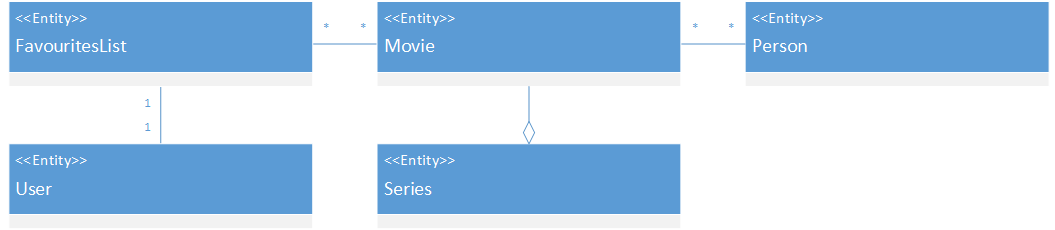
\includegraphics[width=\linewidth]{img/ClassDiagram.png}
\caption{Use case diagram}
\label{fig:use case diagram}
\end{figure}

\subsection{Dynamic model}

\subsubsection{Sequence diagrams}

The sequence diagrams explains some of the more apparant use cases of the system in detail. The interactions shown in the diagrams are not directly linked to the final interaction of the actual program, but is describing the overall flow of the messages sent between the objects being used.

\begin{figure}[H]
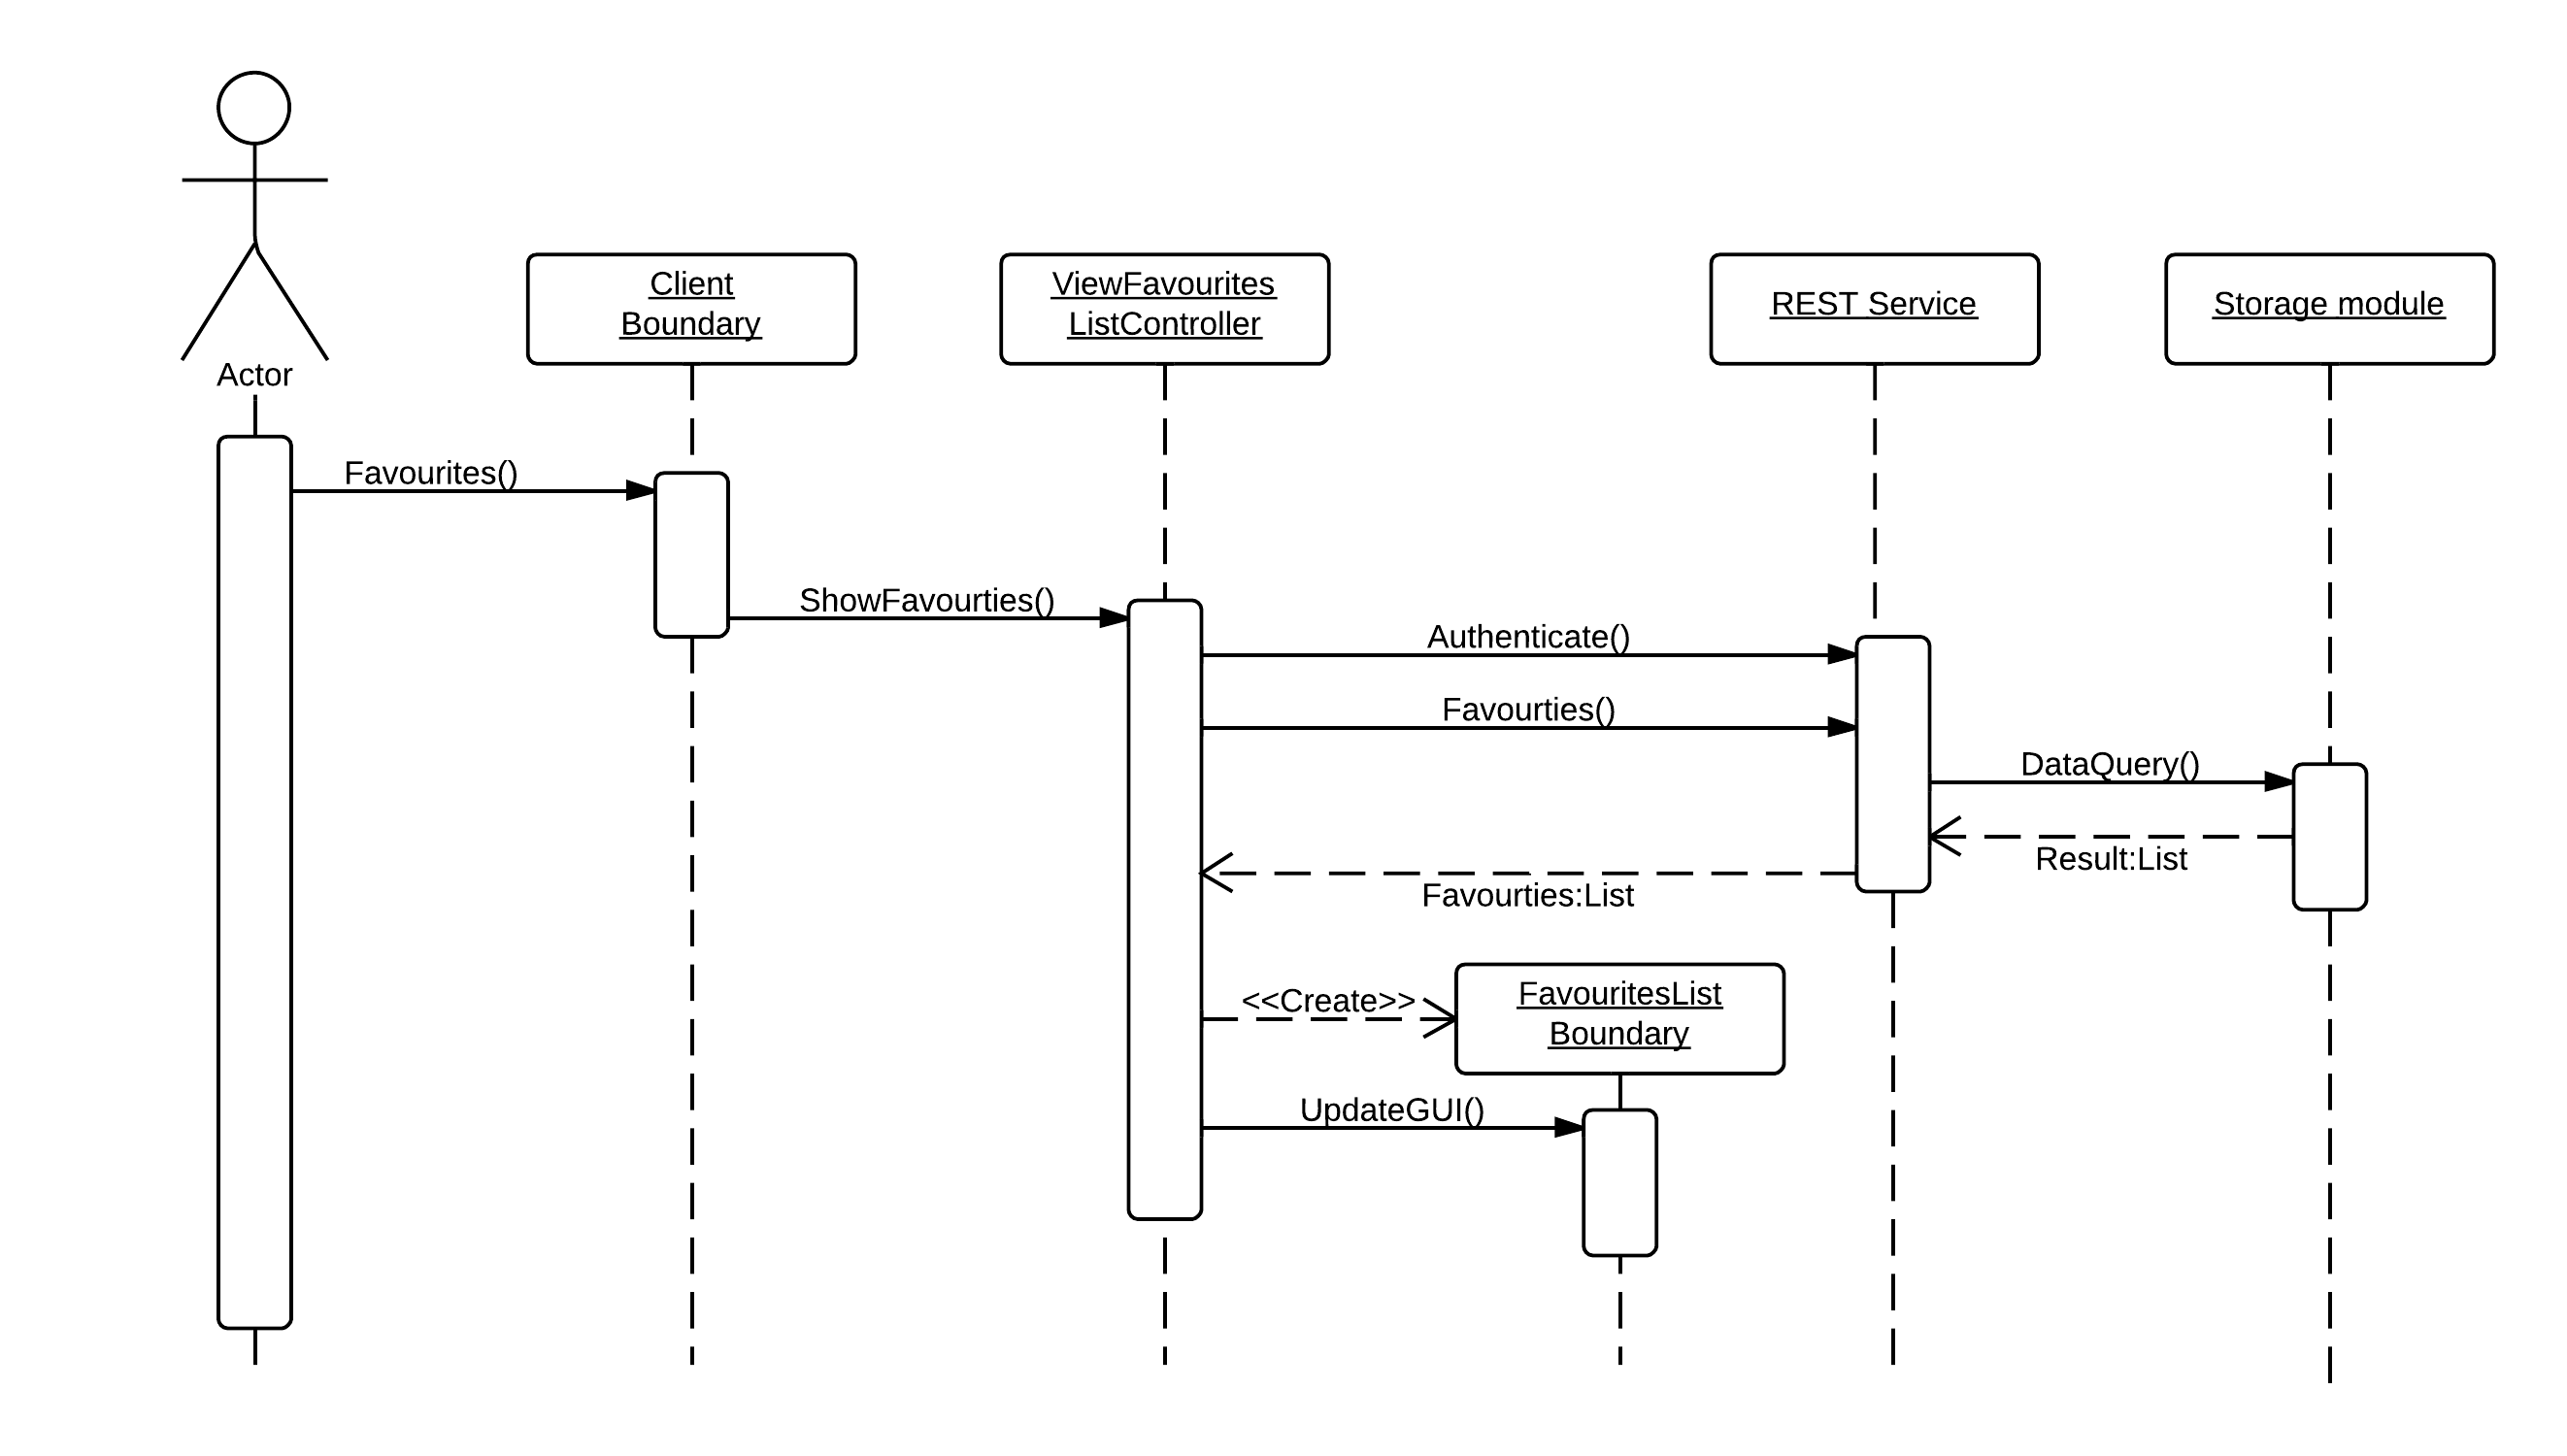
\includegraphics[width=\linewidth]{img/FavouritesSequenceDiagram.png}
\caption{Favourites Sequence Diagram}
\label{fig:Favourites Sequence Diagram}
\end{figure}

\begin{figure}[H]
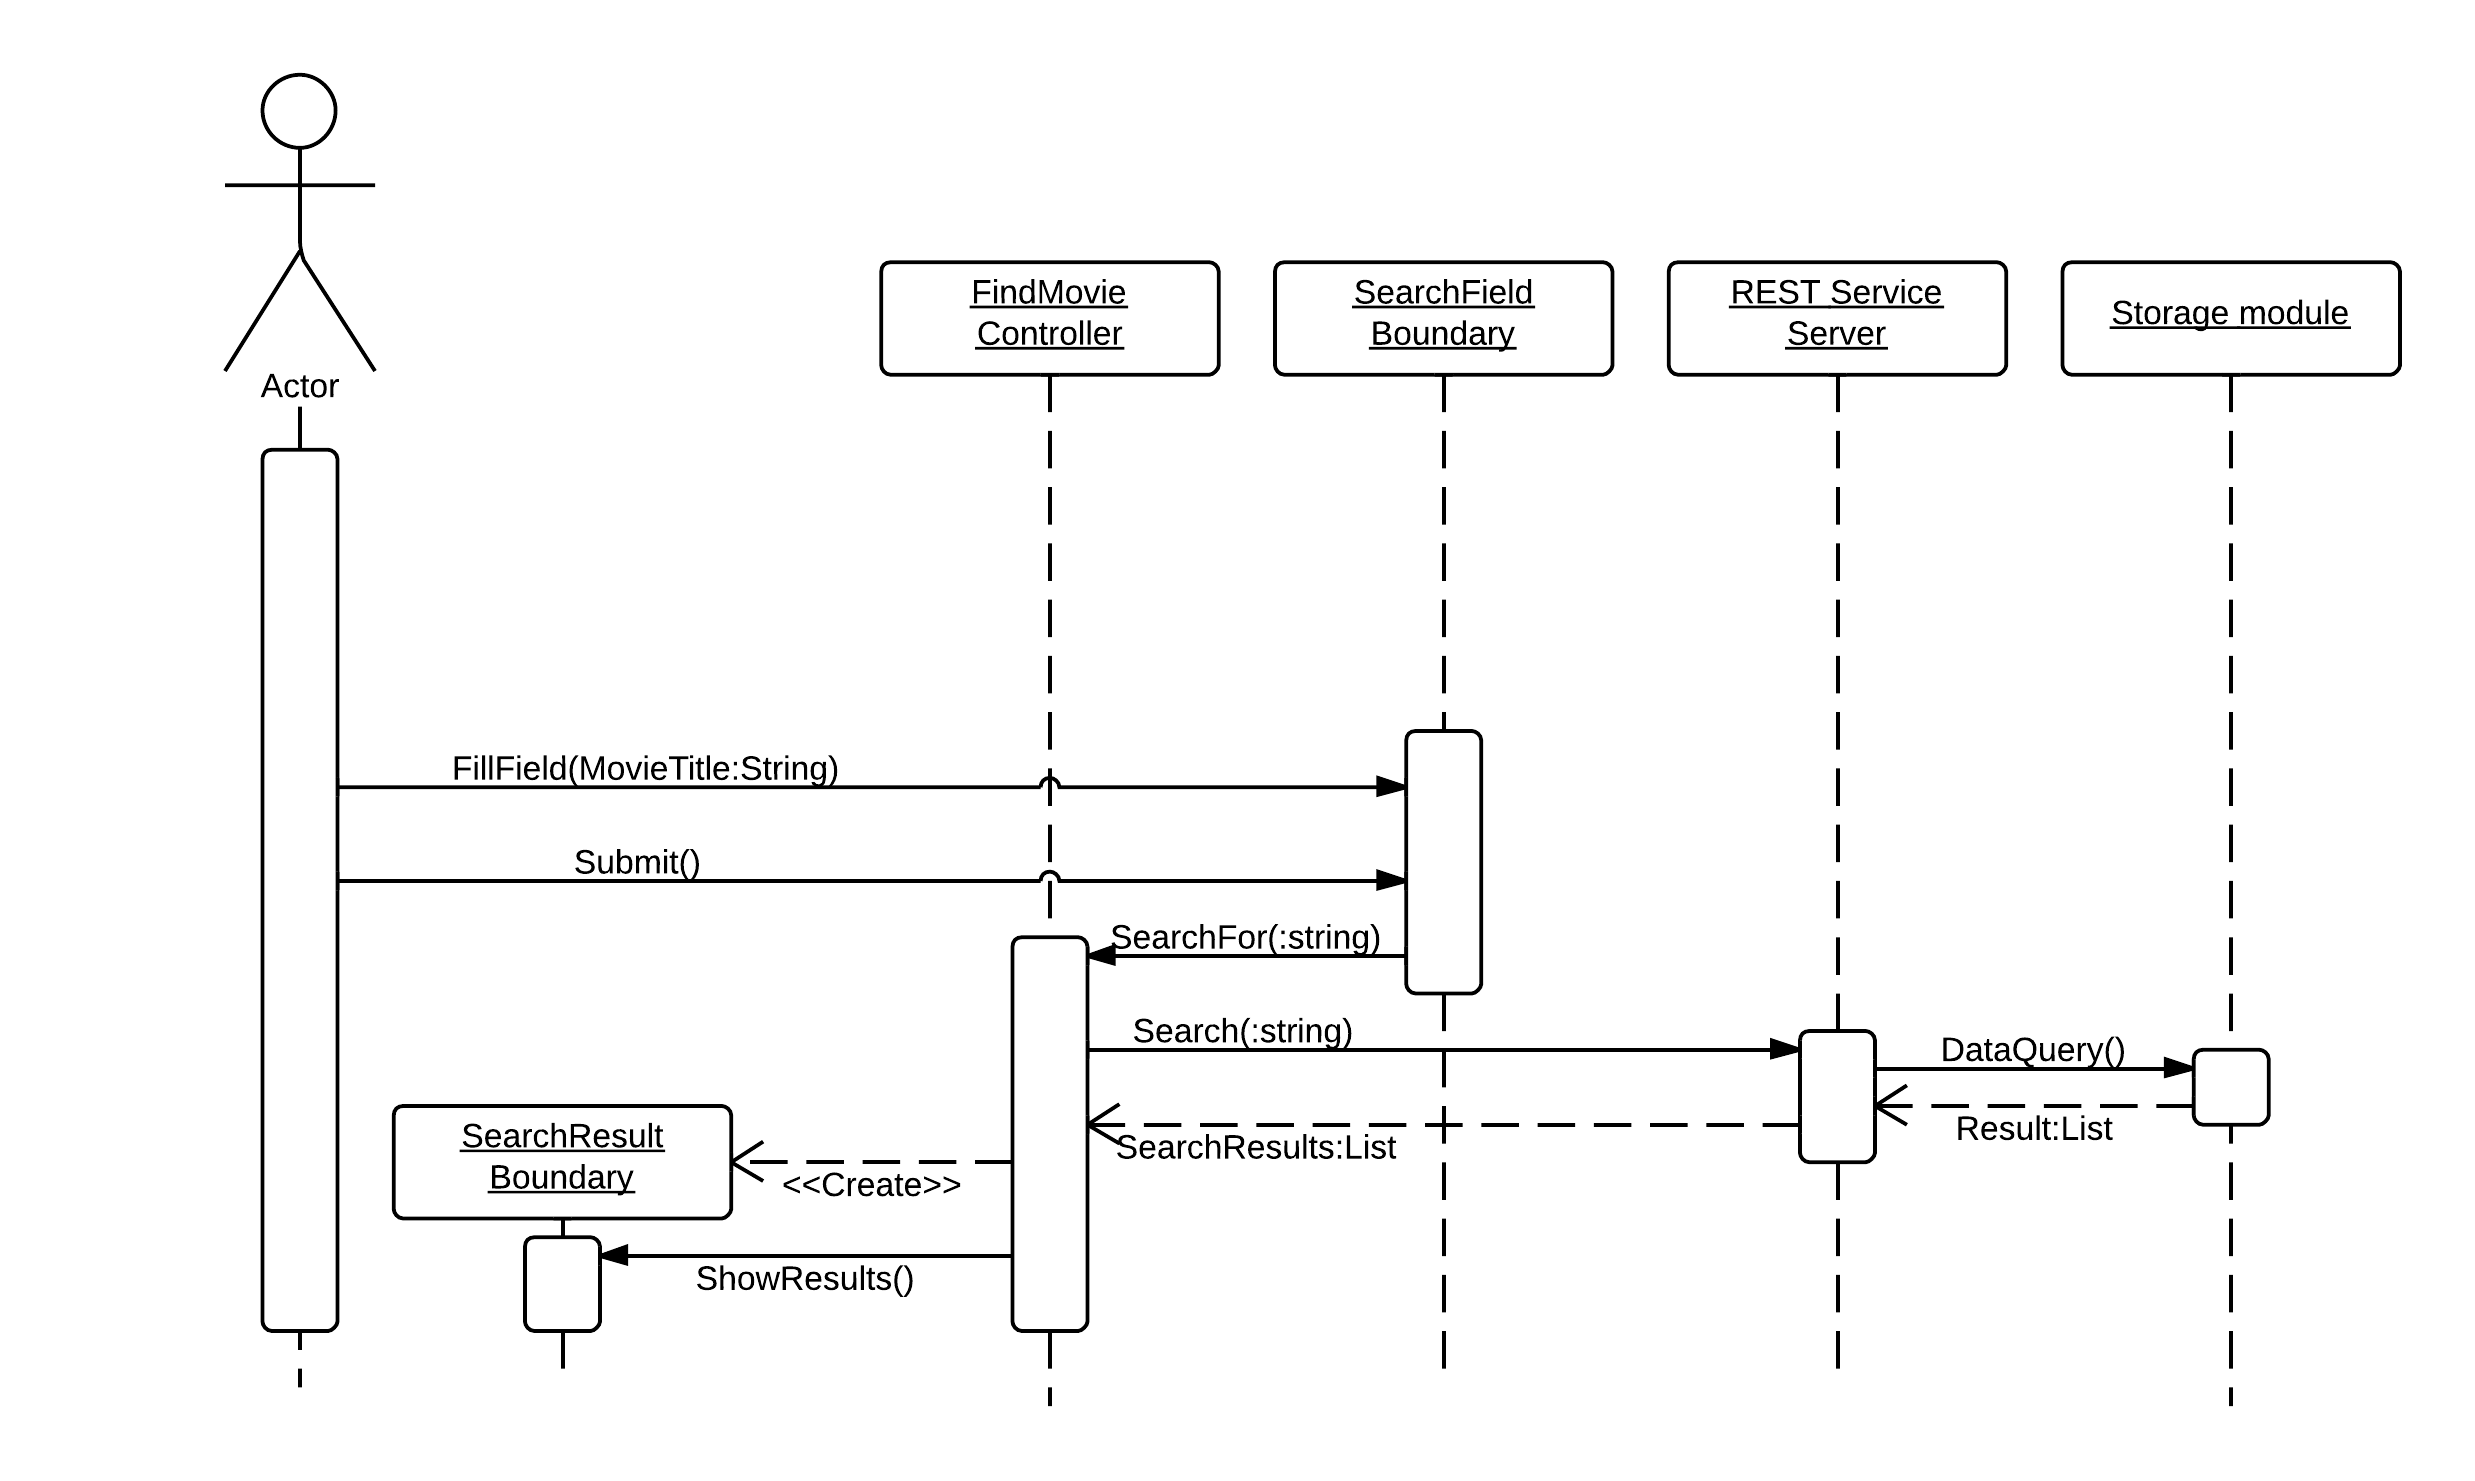
\includegraphics[width=\linewidth]{img/SearchSequenceDiagram.png}
\caption{Search Sequence Diagram}
\label{fig:Search Sequence Diagram}
\end{figure}

\begin{figure}[H]
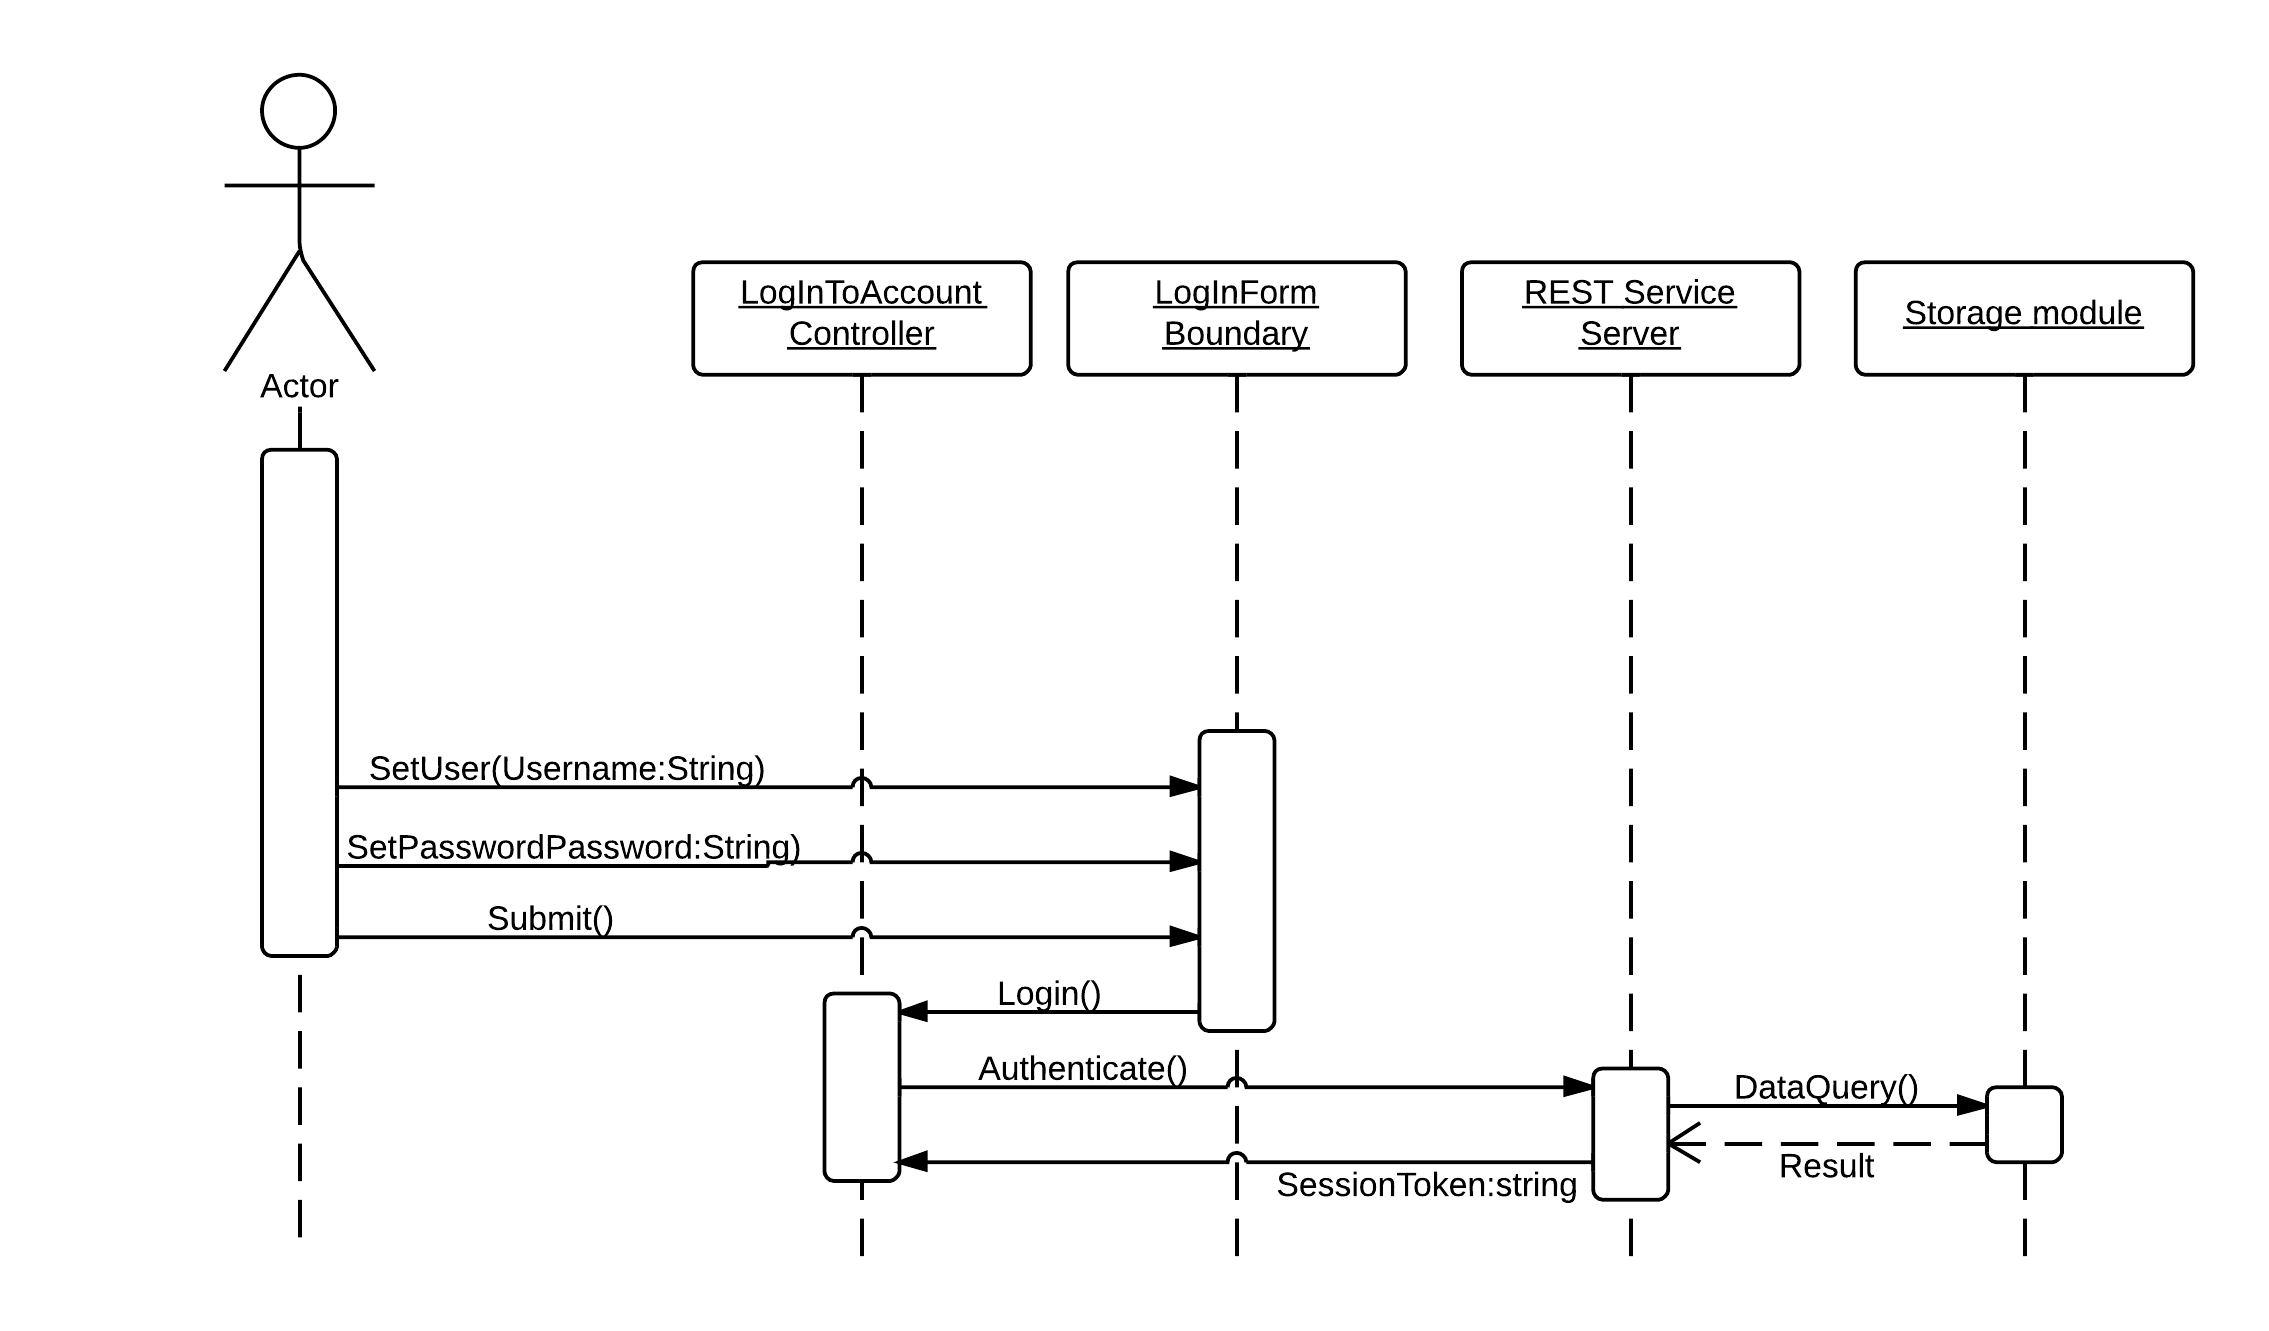
\includegraphics[width=\linewidth]{img/LoginSequenceDiagram.png}
\caption{Login Sequence Diagram}
\label{fig:Login Sequence Diagram}
\end{figure}

\subsubsection{State machines}
An entity can have different states. As seen in figure \ref{fig:Entity State Machine Diagram}, after its creation (POST), it is stores in the persistent database module on the server. From here it can either be deleted (DELETE), or it can be fetched (GET). When a object is queried from the database the server will fetch it as a DTO (Data transfer object) into the servers memory. Often used objects will be saved in the server's cache. The DTO is then sent to the client requesting the object. The client-side also have a cache. This means that if the user has recently queried the object, it will not be fetched from the server, but from the local cache. A DTO can from there either be updated (PUT) and pushed back to the server, or cache time-out and be deleted (This means that only the DTO will be deleted and not the entity in the database).

This is valid for Movies and Actors. Users is not implementing these states as users should not be cached, and only have one state, which is In Database.   

\begin{figure}[H]
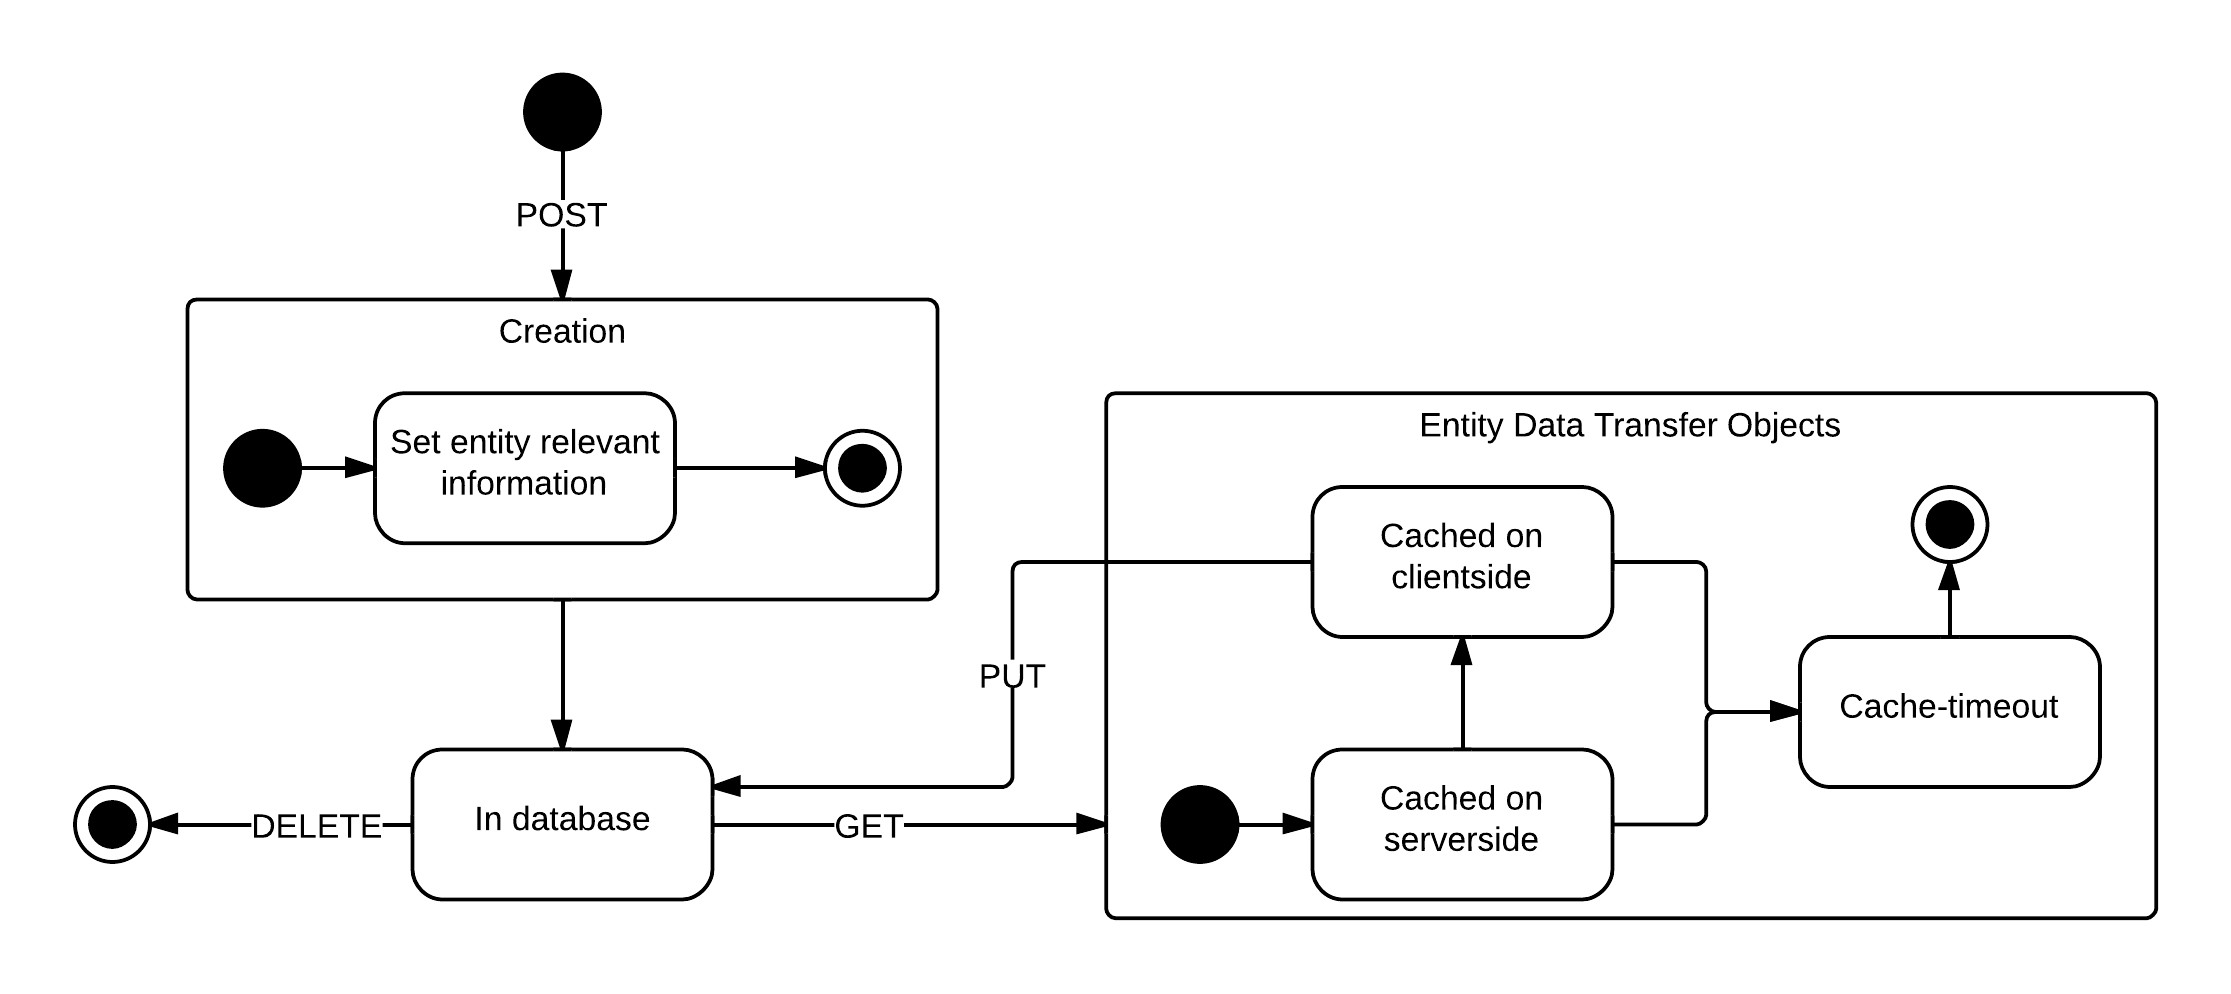
\includegraphics[width=\linewidth]{img/EntityStateMachineDiagram.png}
\caption{Entity State Machine Diagram}
\label{fig:Entity State Machine Diagram}
\end{figure}
\newpage
